\section{Konstruktion des Algorithmus'}

\subsection*{Definitionen und Motivation}

Es gelten die Bezeichnungen des vorherigen Kapitels.
Sei $\Gamma \subset \Lambda$ zudem eine positiv orientierten Jordan-Kurve (d.h. ein geschlossener Weg).
$\Gamma$ umschließe alle Eigenwerte $\lambda_1, \dots, \lambda_k \not \in \Gamma$, und sonst keine weiteren.

\begin{figure}[!ht]
    \centering
    \begin{tikzpicture}

        \draw [->] (-1, 0) -- (9, 0) node [right] {$\Re$};
        \draw [->] (0, -1) -- (0, 5) node [above] {$\Im$};

        \draw (1,   2)   .. controls (1,   1)   and (2,   0.5) ..
              (3,   0.5) .. controls (5,   0.5) and (5,   1.5) ..
              (7,   1.5) .. controls (8,   1.5) and (8.5, 2)   ..
              (8.5, 3)   .. controls (8.5, 4)   and (8,   4.5) ..
              (7,   4.5) .. controls (6,   4.5) and (6,   4)   ..
              (4,   4)   .. controls (3,   4)   and (1,   3.5) ..
              cycle;
        \draw (7.5, 3) node {$\Lambda$};

        \draw (4, 2.5) ellipse [x radius = 2, y radius = 1];
        \draw (4, 3.5) node {$<$};
        \draw (6, 3.5) node {$\Gamma$};

        \filldraw (3, 2.5) circle (1 pt) node [below right] {$\lambda_1$};
        \draw (4, 2.5) node {$\cdots$};
        \filldraw (5, 2.5) circle (1 pt) node [below right] {$\lambda_k$};

    \end{tikzpicture}    
    \caption{$\Lambda$ Gebiet, $\Gamma$ Jordan-Kurve, $\lambda_1, \dots, \lambda_k$ Eigenwerte}
    \label{fig:gebiet_kurve_ews}
\end{figure}

Sei nun $f \in H(\C)$ holomorph.
Wir wenden die Cauchyche Integralformel und den Cauchychen Integralsatz an.
Für $n = 1, \dots, k$, sei dazu $R_n$ hinreichend klein, sodass $B(\lambda_n, R_n) \subset U_n$.

\begin{multline*}
    \implies
    \frac{1}{2 \pi i}
    \Int[\Gamma]
    {
        f(\lambda) A(\lambda)^{-1}
    }{\lambda}
    =
    \frac{1}{2 \pi i}
    \Int[\Gamma]
    {
        f(\lambda)
        \pbraces
        {
            \sum_{n=1}^k
                \frac{1}{\lambda - \lambda_n} P_n^+
                +
                R(\lambda)
        }
    }{\lambda} \\
    =
    \sum_{n=1}^k
        \underbrace
        {
            \frac{1}{2 \pi i}
            \Int[B(\lambda_n, R_n)]
            {
                \frac{f(\lambda)}{\lambda - \lambda_n}
            }{\lambda}
        }_{f(\lambda_n)}
        P_1^+
    +
    \frac{1}{2 \pi i}
    \underbrace
    {
        \Int[\Gamma]
        {
            f(\lambda) R(\lambda)
        }{\lambda}
    }_0
    =
    \sum_{n=1}^k
        f(\lambda_n)
        \sum_{l=n}^{L_n}
            v_{n, l} w_{n, l}^\ast
\end{multline*}

Diese Formel bildet die Grundlage zur Berechnung der Eigenwerte.
Sei $J$ die Summe aller Eigenraum-Dimensionen.
Folgendes würde für lineare Eigenwertprobleme gelten.

\begin{align*}
    J
    :=
    \sum_{n=1}^k
        L_n
    \stackrel{!}{=}
    \sum_{n=1}^k
        \Def(A - I_N \lambda_n)
    =
    \dim
    \bigoplus_{n=1}^k
        \Ker(A - I_N \lambda_n)
    \ll
    \dim \C^N
    =
    N
\end{align*}

Wir vereinigen die Basen all jener (Rechts)-Eigenräume.

\begin{multline*}
    V
    :=
    (V_1, \dots, V_k)
    =
    (v_{1, 1}, \dots, v_{1, L_1}, \dots, v_{k, 1}, \dots, v_{k, L_k}) \\
    =
    \begin{pmatrix}
        v_{1, 1, 1} & \cdots & v_{1, L_1, 1} & \cdots & v_{k, 1, 1} & \cdots & v_{k, L_k, 1} \\
        \vdots      & \ddots & \vdots        & \ddots & \vdots      & \ddots & \vdots        \\
        v_{1, 1, N} & \cdots & v_{1, L_1, N} & \cdots & v_{k, 1, N} & \cdots & v_{k, L_k, N}
    \end{pmatrix}
    \in
    \C^{N \times J}
\end{multline*}

Dasselbe machen wir für die Links-Eigenräume.

\begin{multline*}
    W
    :=
    (W_1, \dots, W_k)
    =
    (w_{1, 1}, \dots, w_{1, L_1}, \dots, w_{k, 1}, \dots, w_{k, L_k}) \\
    =
    \begin{pmatrix}
        w_{1, 1, 1} & \cdots & w_{1, L_1, 1} & \cdots & w_{k, 1, 1} & \cdots & w_{k, L_k, 1} \\
        \vdots      & \ddots & \vdots        & \ddots & \vdots      & \ddots & \vdots        \\
        w_{1, 1, N} & \cdots & w_{1, L_1, N} & \cdots & w_{k, 1, N} & \cdots & w_{k, L_k, N}
    \end{pmatrix}
    \in
    \C^{N \times J}
\end{multline*}

Sei $\hat V \in \C^{N \times j}$ mit $J \leq j \ll N$.

\begin{align} \label{eq:integral_matrizen}
    A_0 := \frac{1}{2 \pi i} \Int[\Gamma]{\lambda^0 A(\lambda)^{-1} \hat V}{\lambda} \in \C^{N \times j},
    \quad
    A_1 := \frac{1}{2 \pi i} \Int[\Gamma]{\lambda^1 A(\lambda)^{-1} \hat V}{\lambda} \in \C^{N \times j}
\end{align}

Sei $D$ die Diagonal-Matrix der Eigenwerte, ihrer Vielfachheit nach aufgeführt.

\begin{align*}
    D
    :=
    \diag
    (
        \underbrace
        {
            \lambda_1, \dots, \lambda_1
        }_{
            \displaystyle
            \text{$L_1$-viele}
        },
        \dots,
        \underbrace
        {
            \lambda_k, \dots, \lambda_k
        }_{
            \displaystyle
            \text{$L_k$-viele}
        }
    )
    =
    \diag(I_{L_1} \lambda_1, \dots, I_{L_k} \lambda_k)
    \in
    \C^{N \times N}
\end{align*}

Das erstere Ergebnis lässt uns nun die Matrix-Integrale $A_0$ und $A_1$ wir folgt umformulieren.
Letztere Gleichheit ist dabei eine elementare, sperrige Rechnung.

\begin{align} \label{eq:integral_matrizen_resultat_compact}
    A_i
    \stackrel{\eqref{eq:integral_matrizen}}{=}
    \frac{1}{2 \pi i}
    \Int[\Gamma]
    {
        \lambda^i
        A(\lambda)^{-1}
        \hat V
    }{\lambda}
    =
    \sum_{n=1}^k
        \lambda_n^i
        \sum_{l=1}^{L_n}
            v_{n, l} w_{n, l}^\ast
    \hat V
    \stackrel{!}{=}
    V D^i W^\ast \hat V,
    \quad
    i = 0, 1
\end{align}

\subsection*{Voraussetzungen}

\begin{enumerate}[label = \arabic*.]

    \item $\lambda_1, \dots, \lambda_k \in \Lambda$ sind alle Eigenwerte.
    Diese sind zudem jeweils halb-einfach und liegen im Inneren von $\Gamma$, d.h. insbesondere nicht darauf.

    \item $V, W \in \C^{N \times J}$ haben vollen Spaltenrang $J$, d.h. deren Spalten linear unabhängig sind.
    Diese Annahme ist sinnvoll.

    $V, W$ bestehen ja schließlich aus Rechts- bzw. Links-Eigenvektoren.
    Die Voraussetzung gilt also zumindest im linearen Fall.
    
    \item $\hat V$ sei eine hinreichend große, gleichverteilt gewählte Zufallsmatrix, mit vollem Spaltenrang $j$.
    Diese Annahme ist sinnvoll.

    Anstelle von $\C$, sei dazu $K$ ein endlicher Körper und $\hat V \in K^{j \times j}$.
    Durch Abzählen der möglichen Komponenten der Spalten der regulären Matrizen, kommt man auf folgende Wahrscheinlichkeit.

    \begin{multline*}
        \mathbf{P}(\hat V \in \GL_j(K))
        =
        \frac
        {
            |\GL_j(K)|
        }{
            |K^{j \times j}|
        }
        =
        \frac{1}
        {
            |K|^{j \cdot j}
        }
        \prod_{i=1}^j
            \pbraces
            {
                |K|^j - |K|^{i-1}
            } \\
        =
        \prod_{i=1}^j
            \frac
            {
                |K|^j - |K|^{i-1}
            }{
                |K|^j
            }
        =
        \prod_{i=1}^j
            \pbraces
            {
                1 - \frac{1}{|K|^{j + 1 - i}}
            }
        \xrightarrow{|K| \to |\C|}
        1
    \end{multline*}

\end{enumerate}

\subsection*{1. Schritt: Konturintegrale}

Nachdem es gilt, $D$ zu bestimmen, bieten $A_0$ und $A_1$ einen Vielversprechenden Anfang.

\begin{align} \label{eq:integral_matrizen_resultat}
    \stackrel
    {
        \eqref{eq:integral_matrizen_resultat_compact}
    }{\implies}
    A_0 = V W^\ast \hat V,
    \quad
    A_1 = V D W^\ast \hat V
\end{align}

Diese werden wir im Wesentlichen durch eine komplexe Variante der Summierten Trapezregel approximieren.
Betrachte dazu folgendes Ringgebiet.

\begin{align*}
    U := \Bbraces{z \in \C: \frac{R}{a_-} < |z| < R a_+},
    \quad
    R > 0,
    \quad
    1 < a_- < a_+
\end{align*}

Wir parametrisieren den Kreis $\partial B(0, R) \subset U$.

\begin{align*}
    \gamma: [0, 1) \to \partial B(0, R): t \mapsto R \exp*{2 \pi i t},
    \quad
    \gamma^\prime: t \mapsto 2 \pi i R \exp*{2 \pi i t}
\end{align*}

Wir approximieren ihn durch die $m$-ten Einheitswurzeln.
Diese wählen wir dann auch als Quadraturknoten, gemeinsam mit gleichmäßigen Gewichten.

\begin{align*}
    \omega_m := \exp \frac{2 \pi i}{m},
    \quad
    m \in \N
\end{align*}

Sei $f \in H(U, \C)$ holomorph.

\begin{multline*}
    Q(f)
    :=
    \frac{1}{2 \pi i}
    \Int[|\lambda| = R]
    {
        f(\lambda)
    }{\lambda}
    =
    \frac{1}{2 \pi i}
    \Int[\gamma]
    {
        f(\lambda)
    }{\lambda}
    =
    \frac{1}{2 \pi i}
    \Int[0][1]
    {
        \gamma^\prime(t)
        f(\gamma(t))
    }{t} \\
    =
    \Int[0][1]
    {
        R
        \exp*{2 \pi i t}
        f(R \exp*{2 \pi i t})
    }{t}
    \approx
    \sum_{\nu = 0}^{m-1}
        \frac{1}{m}
        R \exp \frac{2 \pi i \nu}{m}
        f
        \pbraces
        {
            R \exp \frac{2 \pi i \nu}{m}
        }
    =
    \frac{R}{m}
    \sum_{\nu = 0}^{m-1}
        \omega_m^\nu
        f(R \omega_m^\nu)
    =:
    Q_m(f)
\end{multline*}

$f$ repräsentiert eine Komponente der Integranden von $A_0$ und $A_1$.
Diese müssen vorhin passend zum Ursprung translatiert werden, damit über $\ran \gamma$ anstelle von $\Gamma$ integriert werden kann.
Die (überaus hohe) Genauigkeit der Quadraturformel $Q_m$ wird in ... diskutiert.

Um $A(\lambda)^{-1} \hat V$ in den Integranden von \eqref{eq:integral_matrizen} zu bestimmen, werden wir nicht $A(\lambda)^{-1}$ direkt berechnen.
Stattdessen, bestimmen wir eine LU-Zerlegung von $A(\lambda)$ und führen $j$-mal eine Vorwärts-Rückwärts-Substitution durch.
$\Forall i = 1, \dots, j:$

\begin{align*}
    A(\lambda)^{-1} \hat V_i = x
    \iff
    \hat V_i = A(\lambda) x
\end{align*}

\subsection*{2. Schritt: Singulärwert-Zerlegung}

Wir führen zunächst eine Singulärwert-Zerlegung von $A_0$ durch.

\begin{align*}
    \tilde V \Sigma \tilde W^\ast = A_0 \in \C^{N \times j},
    \quad
    \tilde V \in \U_N(\C),
    \quad
    \tilde W \in \U_j(\C),
    \quad
    \Sigma_{l, k} = \sigma_l \delta_{l, k},
    \quad
    l = 1, \dots, N,
    \quad
    k = 1, \dots, j
\end{align*}

\begin{remark}

    Sei $f \in \Lin(V, W)$ vom Vektorraum $V$ in den Vektorraum $W$, $B \subset V$ eine Basis, und $A$ eine Matrix-Darstellung von $f$.
    Dann gelten folgende Äquivalenzen.

    \begin{multline*}
        \text{$A$ hat vollen Spaltenrang}
        \iff
        \text{$A$ hat linear unabhängige Spalten} \\
        \iff
        \text{$f$ ist injektiv}
        \iff
        \text{$f(B) \subset W$ ist linear unabhängig}
    \end{multline*}

    \begin{multline*}
        \text{$A$ hat vollen Zeilenrang}
        \iff
        \text{$A$ hat linear unabhängige Zeilen} \\
        \iff
        \text{$f$ ist surjektiv}
        \iff
        \text{$f(B) \subset W$ ist Erzeugendensystem}
    \end{multline*}

\end{remark}


Nun haben wir angenommen, dass $V, W \in \C^{N \times J}$ vollen Spaltenrang $J$ haben und $\hat V$ vollen Spaltenrang $j$.
$W^\ast$ hat also vollen Zeilenrang $J$.
Abbildung \ref{fig:rang_1} illustriert, dass $A_0 = V W^\ast \hat V$ genau $J$ linear unabhängige Spalten hat, also Spaltenrang $J$.

\begin{figure}[!ht]
    \centering
    \begin{tikzpicture}[scale = 0.5]

        \draw (0,  0) rectangle (2,  6);
        \draw (6,  0) rectangle (8,  6);
        \draw (12, 0) rectangle (14, 6);
        \draw (18, 0) rectangle (20, 6);

        \draw (0, 1) -- (2, 1);
        \draw (0, 5) -- (2, 5);

        \draw [dotted] (2, 1) -- (6, 0);
        \draw [dotted] (2, 5) -- (6, 6);

        \draw [dotted] (8, 0) -- (12, 2);
        \draw [dotted] (8, 6) -- (12, 4);

        \draw (12, 2) -- (14, 2);
        \draw (12, 4) -- (14, 4);

        \draw [dotted] (14, 2) -- (18, 0);
        \draw [dotted] (14, 4) -- (18, 6);

        \draw (1,  3) node {$\C^j$};
        \draw (4,  3) node {$\xrightarrow[\text{injektiv}]{\hat V}$};
        \draw (7,  3) node {$\C^N$};
        \draw (10, 3) node {$\xrightarrow[\text{surjektiv}]{W^\ast}$};
        \draw (13, 3) node {$\C^J$};
        \draw (16, 3) node {$\xrightarrow[\text{injektiv}]{V}$};
        \draw (19, 3) node {$\C^N$};

    \end{tikzpicture}
    \caption{}
    \label{fig:rang_1}
\end{figure}

Matrizen haben genau dann denselben Rang, wenn sie äquivalent sind.

\begin{align*}
    \begin{pmatrix}
        \diag(\sigma_1, \dots, \sigma_J, \dots, \sigma_j) \\
        0_{(N - j) \times j}
    \end{pmatrix}
    =
    \Sigma
    \equiv
    \tilde V \Sigma \tilde W^\ast
    =
    A_0
    \equiv
    \begin{pmatrix}
        I_J \enspace 0_{J \times (j - J)} \\ 0_{(N - J) \times j}
    \end{pmatrix}
\end{align*}

Damit verschwinden die letzten Singulärwerte $\sigma_{J+1} = \cdots = \sigma_j = 0$.
Somit können wir statt der vollen Singulärwert-Zerlegung (indiziert mit \Quote{full}) eine reduzierte (indiziert mit \Quote{reduced}) verwenden.

\begin{align*}
    A_0
    =
    \tilde V_\mathrm{full} \Sigma_\mathrm{full} \tilde W_\mathrm{full}^\ast
    =
    \begin{pmatrix}
        \tilde V_\mathrm{reduced} & \ast
    \end{pmatrix}
    \begin{pmatrix}
        \Sigma_\mathrm{reduced} & 0_{J \times (j - J)}       \\
        0_{(N - J) \times J}    & 0_{(N - J) \times (j - J)}
    \end{pmatrix}
    \begin{pmatrix}
        \tilde W_\mathrm{reduced}^\ast \\ \ast
    \end{pmatrix}
    =
    \tilde V_\mathrm{reduced} \Sigma_\mathrm{reduced} \tilde W_\mathrm{reduced}^\ast
\end{align*}

Die $\tilde V_\mathrm{full}$ und $\tilde W_\mathrm{full}$ sind ja unitär, d.h. ihre Adjungierten waren ihre Inversen.

\begin{align*}
    \implies
    I_{N \times N}
    =
    \tilde V_\mathrm{full}^\ast \tilde V_\mathrm{full}
    =
    \begin{pmatrix}
        \tilde V_\mathrm{reduced}^\ast \\ \ast
    \end{pmatrix}
    \begin{pmatrix}
        \tilde V_\mathrm{reduced} & \ast
    \end{pmatrix}
    =
    \begin{pmatrix}
        \tilde V_\mathrm{reduced}^\ast \tilde V_\mathrm{reduced} & \ast \\
        \ast                                                     & \ast
    \end{pmatrix}
\end{align*}

Eine analoge Rechnung kann man, mit $j$ anstelle von $N$, für $\tilde W_\mathrm{reduced}$ machen.
Insgesamt erhalten wir also folgende Tatsachen über unsere reduzierte Singulärwert-Zerlegung.
Wir vereinbaren, ab sofort nur noch die reduzierte Singulärwert-Zerlegung zu verwenden und den Index wegzulassen.

\begin{align} \label{eq:singulärwert_zerlegung}
    \tilde V^\ast \tilde V
    =
    \tilde W^\ast \tilde W
    =
    I_{J \times J},
    \quad
    \Sigma = \diag(\sigma_1, \dots, \sigma_J),
    \quad
    A_0 = \tilde V \Sigma \tilde W^\ast
\end{align}

$\tilde V$ hat, als Teil-Matrix einer unitären, vollen Spaltenrang $J$ hat.
$\tilde V^\ast$ hat also vollen Zeilenrang $J$.
Abbildung \ref{fig:rang_2} illustriert, dass $S := \tilde V^\ast V \in \C^{J \times J}$ genau $J$ linear unabhängige Spalten hat, also $S \in \GL_J(\C)$.

\begin{figure}[!ht]
    \centering
    \begin{tikzpicture}[scale = 0.5]

        \draw (0,  0) rectangle (2,  6);
        \draw (6,  0) rectangle (8,  6);
        \draw (12, 0) rectangle (14, 6);

        \draw (0, 2) -- (2, 2);
        \draw (0, 4) -- (2, 4);

        \draw [dotted] (2, 2) -- (6, 0);
        \draw [dotted] (2, 4) -- (6, 6);

        \draw [dotted] (8, 0) -- (12, 2);
        \draw [dotted] (8, 6) -- (12, 4);

        \draw (12, 2) -- (14, 2);
        \draw (12, 4) -- (14, 4);

        \draw (1,  3) node {$\C^J$};
        \draw (4,  3) node {$\xrightarrow[\text{injektiv}]{V}$};
        \draw (7,  3) node {$\C^N$};
        \draw (10, 3) node {$\xrightarrow[\text{surjektiv}]{\tilde V^\ast}$};
        \draw (13, 3) node {$\C^J$};

    \end{tikzpicture}
    \caption{}
    \label{fig:rang_2}
\end{figure}

In den folgenden Gleichungsketten wird bei \Quote{!} die jeweils vorgerige eingesetzt.

\begin{align*}
    & \implies
    \Sigma \tilde W^\ast
    \stackrel
    {
        \eqref{eq:singulärwert_zerlegung}
    }{=}
    \tilde V^\ast \tilde V \Sigma \tilde W^\ast
    \stackrel
    {
        \eqref{eq:singulärwert_zerlegung}
    }{=}
    \tilde V^\ast A_0
    \stackrel
    {
        \eqref{eq:integral_matrizen_resultat}
    }{=}
    \tilde V^\ast V W^\ast \hat V
    =
    S W^\ast \hat V \\
    & \implies
    A_1
    \stackrel
    {
        \eqref{eq:integral_matrizen_resultat}
    }{=}
    V D W^\ast \hat V
    \stackrel{!}{=}
    V D S^{-1} \Sigma \tilde W^\ast \\
    & \implies
    \tilde V^\ast A_1 \tilde W \Sigma^{-1}
    \stackrel{!}{=}
    \tilde V^\ast V D S^{-1} \Sigma \tilde W^\ast \tilde W \Sigma^{-1}
    =
    S D S^{-1}
    \approx
    D
\end{align*}

Somit ist die Diagonalmatrix $D$, welche ja die gesuchten Eigenwerte enthält, ähnlich zur Matrix $\tilde V^\ast A_1 \tilde W \Sigma^{-1}$.
Ähnliche Matrizen haben dieselben Eigenwerte.

\subsection*{Zusammenfassung}

Wir haben insgesamt den folgenden Algorithmus \ref{alg:integral_methode_zusammenfassung} gefunden.

\begin{algorithm}[H]
	\label{alg:integral_methode_zusammenfassung}
	\caption{Integral-Methode}
    \begin{algorithmic}[1]
        \Procedure{Integral-Methode Zusammanfassung}{}
            \State Berechne $A_0, A_1 \in \C^{N \times j}$ (z.B. mit LU-Zerlegung);
            \State Berechne und reduziere eine Singulärwert-Zerlegung $A_0 = \tilde V \Sigma \tilde W^\ast$ auf $J$ Singulärwerte;
            \State Berechne Eigenwerte $\lambda_1, \dots, \lambda_k$ der Matrix $\tilde V A_1 \tilde W \Sigma^{-1}$ (z.B. mit QR-Verfahren);
            \State \Return $\lambda_1, \dots, \lambda_k$
		\EndProcedure
	\end{algorithmic}
\end{algorithm}
